% Part: sets-functions-relations
% Chapter: arithmetization
% Section:reals
% Hindi translation (hi-Deva-IN) of Open Logic commit 9620cc73f9c8e0ad003c514a5d3748f29611c4c0.

\documentclass[../../../include/open-logic-section]{subfiles}

\begin{document}

\olfileid[hi]{sfr}{arith}{real}
\olsection{वास्तविक संख्या-रेखा}

अगला चरण यह दिखाना है कि परिमेय संख्याओं से वास्तविक संख्याएँ कैसे बनाई जाती
हैं। उससे पहले हमें समझना होगा कि वास्तविक संख्याओं की
\emph{विशिष्टता} क्या है।

वास्तविक संख्याएँ बहुत कुछ परिमेय संख्याओं जैसा व्यवहार करती हैं। (तकनीकी
रूप से दोनों \emph{क्रमित क्षेत्रों} के उदाहरण हैं; इसकी परिभाषा के लिए
\olref[check]{orderedfield} देखें।) यदि आपने \olref[sfr][siz][]{chap} के
अभ्यास किए हैं, तो आप जानते होंगे कि वास्तविक संख्याओं की संख्या परिमेय
संख्याओं की संख्या से अधिक है, अर्थात $\cardless{\Rat}{\Real}$। इसका पहला प्रमाण कैंटर ने
दिया था। लेकिन लगभग ढाई सहस्राब्दियों से यह ज्ञात है कि अपरिमेय संख्याएँ भी
होती हैं, अर्थात ऐसी वास्तविक संख्याएँ जो परिमेय नहीं हैं। वास्तव में:
%\footnote{Now: ``$\sqrt{2}$'' equally refers to both the positive and the negative roots; but in the next few pages, I'll forget about this, and consider only the positive root.}
\begin{thm}\ollabel{root2irrational}
$\sqrt{2}$ परिमेय नहीं है, अर्थात $\sqrt{2} \notin \Rat$।
\end{thm}

\begin{proof}
प्रतिविरोध के लिए मान लें कि $\sqrt{2}$ परिमेय है। तब $\sqrt{2} =
\nicefrac{m}{n}$, जहाँ $m$ और $n$ कुछ प्राकृत संख्याएँ हैं। हम $m$ और $n$
को ऐसा चुन सकते हैं कि भिन्न को इससे अधिक
सरल न किया जा सके। पदों को पुनर्व्यवस्थित करने पर $m^{2} = 2n^{2}$। यहाँ से
प्रमाण दो ढंग से पूरा किया जा सकता है:

\emph{पहला, ज्यामितीय ढंग से} (टेनेनबाउम का अनुसरण करते हुए)।\footnote{यह
प्रमाण \cite{Conway2006} में दिया गया है।} इन वर्गों पर विचार करें:
\begin{center}	
	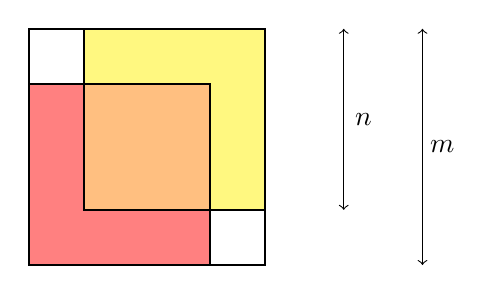
\begin{tikzpicture}
		\draw[thick] (0,0) rectangle (3,3);
		\draw[thick, fill=red!50] (0,0) rectangle (2.3,2.3);
		\draw[thick, fill=yellow!50] (0.7,0.7) rectangle (3, 3);
		\draw[thick, fill=orange!50] (0.7,0.7) rectangle (2.3, 2.3);
		\draw[<->] (4, 0.7)--(4, 3);
		\node at (4.25, 1.85) (n) {$n$};
		\draw[<->] (5, 0)--(5, 3);
		\node at (5.25, 1.5) (m) {$m$};
	\end{tikzpicture}
\end{center}
चूँकि $m^2 = 2n^2$, इसलिए $n$ भुजा वाले दोनों वर्गों का अतिव्याप्त क्षेत्र
उतना ही है जितना वह क्षेत्र जिसे दोनों में से कोई वर्ग नहीं ढकता; अर्थात
नारंगी वर्ग का क्षेत्रफल दोनों बिना रंगे वर्गों के कुल क्षेत्रफल के बराबर है।
अतः यदि नारंगी वर्ग की भुजा $p$ और प्रत्येक बिना रंगे वर्ग की भुजा $q$ हो, तो
$p^2 = 2q^2$। किंतु अब $\sqrt{2} = \nicefrac{p}{q}$, जहाँ $p < m$, $q < n$
और $p, q \in
\Nat$। यह इस तथ्य का खंडन करता है कि $m$ और $n$ को यथासंभव छोटा चुना गया था।
		
\emph{दूसरा, बीजगणितीय ढंग से।} चूँकि $m^{2} = 2n^{2}$, इसलिए $m$ सम है।
(यह दिखाना आसान है कि यदि $x$ विषम हो, तो $x^2$ भी विषम होता है।) अतः
$m = 2r$, जहाँ $r \in \Nat$। पुनर्व्यवस्थित करने पर $2r^2 = n^2$,
		%\begin{align*}
		%\t(2q)^{2} &= 2n^{2}\\
		%\t4q^{2} &= 2n^{2}\\
		%\t2q^{2} &= n^{2}
		%\end{align*}
इसलिए $n$ भी सम है। इस प्रकार $m$ और $n$ दोनों सम हैं, और फलतः भिन्न
$\nicefrac{m}{n}$ को \emph{और} सरल किया जा सकता है। यह प्रतिविरोध है!
\end{proof}

प्रसंगवश, यह आरेखीय प्रमाण हमें \olref[his][set][mythology]{sec} की सामग्री
पर फिर से विचार करने देता है। टेनेनबाउम (1927--2006) पूरी तरह आधुनिक गणितज्ञ
थे; फिर भी यह प्रमाण निस्संदेह सुंदर, पूर्णतः कठोर और ज्यामितीय अंतर्ज्ञान पर
आधारित है!

बहरहाल, वास्तविक संख्याएँ परिमेय संख्याओं से ``अधिक विस्तृत'' हैं। एक अर्थ
में परिमेय संख्या-रेखा में ``रिक्त स्थान'' हैं, जिन्हें वास्तविक संख्याएँ भरती
हैं। वाइयरश्ट्रास ने समझा कि यह वास्तविक संख्याओं के एक ही गुणधर्म का वर्णन
है, जो उन्हें परिमेय संख्याओं से अलग करता है---पूर्णता गुणधर्म: \emph{वास्तविक
संख्याओं के प्रत्येक रिक्तेतर समुच्चय का, यदि वह ऊपर से परिबद्ध हो, तो एक
लघुतम ऊपरी परिबंध होता है।}

यह देखना आसान है कि परिमेय संख्याओं में पूर्णता गुणधर्म नहीं होता। उदाहरण के
लिए $\sqrt{2}$ से छोटी परिमेय संख्याओं के इस समुच्चय पर विचार करें:
\[
	\Setabs{p \in \Rat}{p^2 < 2 \text{ अथवा }p < 0}
\]
परिमेय संख्याओं में इसका एक ऊपरी परिबंध है; उदाहरण के लिए इसके सभी
!!{element} $3$ से छोटे हैं। किंतु इसका लघुतम ऊपरी परिबंध क्या है? हम
`$\sqrt{2}$' कहना चाहते हैं; पर अभी देखा है कि $\sqrt{2}$ परिमेय
\emph{नहीं} है। और $\sqrt{2}$ से बड़ी कोई \emph{लघुतम} परिमेय संख्या नहीं
है। अतः इस समुच्चय का ऊपरी परिबंध तो है, पर लघुतम ऊपरी परिबंध नहीं। इसलिए
परिमेय संख्याओं में पूर्णता गुणधर्म का अभाव है।

इसके विपरीत, अविच्छिन्न संख्या-रेखा में पूर्णता गुणधर्म ``होना ही चाहिए''। हम
केवल $\sqrt{2}$ को वास्तविक संख्या नहीं बनाना चाहते; हम परिमेय संख्या-रेखा के
सभी ``रिक्त स्थान'' भरना चाहते हैं। वास्तव में हम चाहते हैं कि अविच्छिन्न रेखा
में स्वयं कोई ``रिक्त स्थान'' न रहे। पूर्णता के माध्यम से हमें ठीक यही मिलेगा।

\end{document}
